\documentclass{article}

\usepackage[left=2cm,right=2cm, top=2cm, bottom = 2cm]{geometry}
\usepackage{amsfonts}
\usepackage{amsmath}
\usepackage{amssymb}
%%%\usepackage{array}

\usepackage{tikz}

\pagestyle{empty}

\usepackage{xcolor}
\usepackage{fancyvrb}

\begin{document}

\title{Graphs, Recursion, and Induction}
\date{}

\maketitle
\thispagestyle{empty}

\Large

\textbf{\underline{Objective: To understand how to use induction to prove statements}}

\textbf{\underline{about graphs, and relate it to recursive programs.}}


\vspace{5mm}


\textbf{Proof by Induction \& Euclid's Algorithm:}\bigskip



Induction can be thought of as the proof version of recursion in computer science. We will explore this idea, and see how proving statements like induction can be similar to writing a program that uses recursion.\medskip

The \textbf{highest common factor} (hcf) of two non-negative integers $a$ and $b$ is the largest number $h$ such that $a=h\alpha$ and $b=h\beta$ for some integers $\alpha$ and $\beta$. Euclid's algorithm is a classical method for finding the hcf of two numbers. In Python:
\begin{Verbatim}
def euclid(a, b):
	if a < b:
		return euclid(b, a)  # want bigger one first
	if b == 0:
		return a  # base case
	
	# now some code to write a = (b * quotient) + remainder,
	# where remainder < b
	quotient = 0
	remainder = a
	new_remainder = a - b
	while new_remainder >= 0:
		remainder = new_remainder
		quotient += 1
		new_remainder -= b
	
	return euclid(b, remainder)  # recursive step
\end{Verbatim}


Why does this necessarily return $\mathrm{hcf}(a,b)$? We will prove it by induction on $b$, in parallel with the recursion in the code.

Induction has two parts; a \textbf{base case} and an \textbf{inductive step}. For the base case, we deal with the smallest possible value of the inductive variable (in this case, $b$). This is like establishing a base case for a recursive program, so the recursion will eventually terminate. In this case, the base case is $b=0$.

The inductive step then corresponds to the recursive call of the function; when writing a recursive piece of code, you assume your code can handle a ``smaller'' input than it currently has, so your job is to reduce the problem with the current input to solving the problem with a smaller input, which you can then do by calling your code recursively. In induction, you assume you have proved the result for smaller inputs, so your job is to reduce the problem with the current input to solving the problem with a smaller input, which you then do by referring to your proof recursively (using the \textbf{inductive hypothesis}).

Let's see this in action when proving that Euclid's algorithm returns the highest common factor of its inputs:

\begin{enumerate}
	\item Prove the base case. In other words, prove that if $b=0$, $\mathrm{euclid}(a, 0)$ returns the hcf of $a$ and 0.
\end{enumerate}

Now we need to prove the inductive step. In other words, assume that for any $c<b$, $\mathrm{euclid}(a,c)$ returns the hcf of $a$ and $c$, and prove that $\mathrm{euclid}(a,b)$ returns the hcf of $a$ and $b$. This step is harder, so we need to break it down further:

\begin{enumerate}\setcounter{enumi}{1}
	\item Show that $\mathrm{euclid}(a,b)$ returns $\mathrm{euclid}(b,r)$, where $r$ is the remainder when $a$ is divided by $b$. This means that
		\[a=bq+r,\]
		where $0\leq r < b$.
\end{enumerate}

Now we know by the inductive step (our recursion) that $\mathrm{euclid}(b,r)$ is the hcf of $b$ and $r$, so we just need to show that $\mathrm{hcf}(b,r)=\mathrm{hcf}(a,b)$. Let $h=\mathrm{hcf}(b,r)$; we need to show that $h$ is the highest common factor of $a$ and $b$. We know two things about $h$: firstly, it is a common factor of $b$ and $r$, and secondly, if $h'$ is a common factor of $b$ and $r$, then $h'\leq h$. We want to show two more things about $h$: that $h$ is a common factor of $a$ and $b$, and that if $h'$ is a common factor of $a$ and $b$, then $h'\leq h$. Clearly, we should use each property we know about $h$ to prove the corresponding property we want.

\begin{enumerate}\setcounter{enumi}{2}
	\item Show that $h$ is a common factor of $a$ and $b$, using the fact that $h$ is a common factor of $b$ and $r$.
	\item Show that if $h'$ is any common factor of $a$ and $b$, then $h'\leq h$, using the corresponding fact for $b$ and $r$.
\end{enumerate}

\bigskip

So what does any of this have to do with graphs? Well, we can define a directed graph $G$ as follows: the vertices of $G$ are non-negative integers, and there is an edge $u\to v$ if $u$ divides $v$---\textit{i.e.}, if $v=un$ for some $n\geq 1$. Part of this graph looks like this (with loops at each vertex not drawn):
\begin{center}
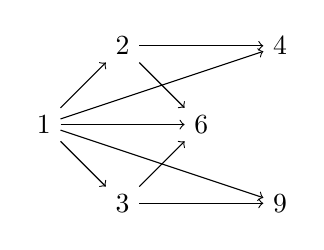
\begin{tikzpicture}
	\node (1) at (0,0) {1};
	\node (2) at (1,1) {2};
	\node (3) at (1,-1) {3};
	\node (6) at (2,0) {6};
	\node (4) at (3,1) {4};
	\node (9) at (3,-1) {9};
	
	\draw
		(1) edge[->] (2)
		(2) edge[->] (6)
		(1) edge[->] (3)
		(1) edge[->] (6)
		(3) edge[->] (6)
		(1) edge[->] (4)
		(2) edge[->] (4)
		(1) edge[->] (9)
		(3) edge[->] (9)
	;
\end{tikzpicture}
\end{center}

Note that the graph is infinite. There is an edge from 1 to every vertex, and an edge from every vertex to 0. The prime numbers are the vertices which are the target of only two edges (the one from 1 and the one from the vertex to itself). The hcf of two numbers $a$ and $b$ is the unique vertex $h$ such that there are edges $h\to a$ and $h\to b$, and whenever $h'$ is a vertex with edges $h'\to a$ and $h'\to b$, then there is an edge $h'\to h$; if we think of all arrows as going left-to-right, then $h$ is the right-most vertex that has an arrow to both $a$ and $b$; a lattice-theorist would call this the ``infimum'' of $a$ and $b$.

So Euclid's algorithm gives a way of finding the vertex furthest to the right which has edges to both $a$ and $b$ (the infimum of $a$ and $b$; it does this by finding $r$ further to the left than $b$ such that the infimum of $b$ and $r$ is the same as the infimum of $a$ and $b$.

\clearpage




\textbf{Vertex Colourings:}\bigskip


Suppose $G$ is a finite simple graph (with complement $\bar{G}$) and we want to prove a statement like
\[\chi(G)+\chi(\bar{G})\leq |G|+1.\]

Since $\chi(G)$ is the minimum number of colours needed to colour $G$, we might imagine trying to write some code to compute $\chi(G)$. We'll imagine doing this recursively; the analogy between recursive programming and proof by induction should then allow us to prove the above statement.

So our program will take a graph $G$, find some way to break it down into a smaller graph $H$ (or maybe several smaller pieces), call itself recursively to find $\chi(H)$, then figure out how to go from $\chi(H)$ back to $\chi(G)$. We won't actually be able to do this, but by trying to, we'll be able to prove the inequality above. We need a base case so that our recursion will terminate; so we need to figure out how to compute $\chi(G)$ for a really small graph $G$ (and check that it satisfies the inequality above). So we start with a graph having just a single vertex, and establish that as our base case.\medskip

Then for our inductive step (when we call our program recursively), we need to figure out how we're going to break $G$ up into one or more smaller graphs, and how to put those pieces back together to find $\chi(G)$ (or at least estimate it, so as to get the inequality we're actually trying to prove). So we assume our program can handle any graph with at most $n$ vertices (ideally, we want our program to be able to compute $\chi(G)$ for any small enough graph, but maybe the best we can hope for is that we can prove the above inequality for any smaller graph). Now we take a graph $G$ with $n+1$ vertices, and think how to break it up.

The easiest thing to do is to pick a single vertex, $v$, and remove it; so let $H=G\setminus v$; then $G$ has $n$ vertices, so our hypothetical program can find $\chi(H)$; for our induction, what this means is that we know that
\[\chi(H)+\chi(\bar{H})\leq n+1.\]
We now need to figure out how putting $v$ back in affects $\chi$, to work out what $\chi(G)$ is---or rather, to prove that
\[\chi(G)+\chi(\bar{G})\leq n+2.\]

The problem is that we don't know how many edges connect to $v$ in $G$, and this will affect how we can colour $G$. Suppose our recursive call to the program gives us a $\chi(H)$-colouring of $H$; how can we extend this to a colouring of $G$? Under what circumstances will we need an extra colour? And how about taking a colouring of $\bar{H}$, and extending that? When will we need an extra colour there?\bigskip


Let's first prove an easier problem (this is often a useful trick when stuck on a proof). Prove that
\[\chi(G)+\chi(\bar{G})\leq |G|+2.\]
To do this, set up a base case (actually, the same as before!), assume the result holds when $|G|\leq n$, and then take $G$ with $n+1$ vertices, take a vertex off, and think about the ``worst case'' when adding that vertex back in.





\end{document}